\chapter{\color{oxfordblue} The LHC \& ATLAS Experiment}\label{chapter-ATLAS}
\ChapFrame

\textit{
Modern particle physics explores the frontier of the technological reach of science. To discover the Higgs boson, a remarkably complex infrastructure is necessary to probe physics at the required scale. The \gls{cern} hosts the largest and most powerful particle accelerator ever built: the Large Hadron Collider. It has held this title since its construction concluded in 2008 \cite{LyndonEvans_2008}, and easily ranks as one of the most intricate machines ever created. Protons are accelerated to up to 99.9999991\% of the speed of light in its giant 27 km long ring-shaped beamline, buried 100 m below the surface of the French-Swiss border in the suburb of Geneva. Superconducting magnets cooled down with liquid helium to 1.9 $K$ steer this energetic beam thanks to powerful magnetic fields of 8.33 Tesla. The beams, composed of bunches of particles, are collided at four precise interaction points where large detectors are built and operated by dedicated collaborations: ATLAS \cite{TheATLASCollaboration_2008}, CMS \cite{TheCMSCollaboration_2008}, ALICE \cite{TheALICECollaboration_2008}, and LHC$b$ \cite{TheLHCbCollaboration_2008}. The first two are multipurpose experiments with overlapping physics programs, while ALICE and LHC$b$ respectively study heavy ion and heavy flavour physics. This chapter describes the experimental setup of the \gls{lhc} and the ATLAS experiment, focusing on proton-proton collisions and introducing relevant elements for the work presented in this thesis.} 

\section{The Large Hadron Collider}\label{sec-LHC}
The last machine in the complex multi-stage accelerator complex of CERN depicted in Figure \ref{fig-CernAccSys}, the \glsfirst{lhc} is capable of frontally colliding proton or heavy ion beams packed into bunches. The beams collide at four interaction points, where dedicated experiments such as ATLAS measure the resulting physics signatures in large detectors designed for their specific physics programmes. The life of a proton beam starts in a bottle of ionised hydrogen $H^-$ gas, the content of which is passed through a linear accelerator called \textsc{linac} 4\footnote{\textsc{linac} 2 before 2020.} to reach energies of 160 MeV \cite{Vretenar:2020quc}. After stripping the ionised hydrogen atoms of their two electrons to leave bare protons, the next acceleration stage happens in the Proton Synchrotron Booster (\textsc{booster}), bringing the beam energy to 2 GeV \cite{Reich:1969fw}. The protons are then handed to increasingly larger synchrotrons: the Proton Synchrotron (\textsc{ps}) to reach energies of 26 GeV \cite{CERNPS}, followed by the Super Proton Synchrotron (\textsc{sps}) to reach energies of 450 GeV \cite{Synchrotron:1997188}. The beam is finally injected into the \gls{lhc} in two different beamlines circulating the proton in opposite directions \cite{Evans:2008zzb}. Superconducting dipole magnets generating a 8.33 T field steer the highly energetic beams, while complex geometries of magnets such as quadrupoles and sextupoles refine the bunch shape through focusing effects. Powerful radiofrequency cavities accelerate the protons to their final energy of 6.5 TeV, giving a total $pp$ collision centre-of-mass energy of $\sqrt{s} = 13$ TeV in Run 2. 

\begin{figure}[!h]
  \centering
  \makebox[\textwidth][c]{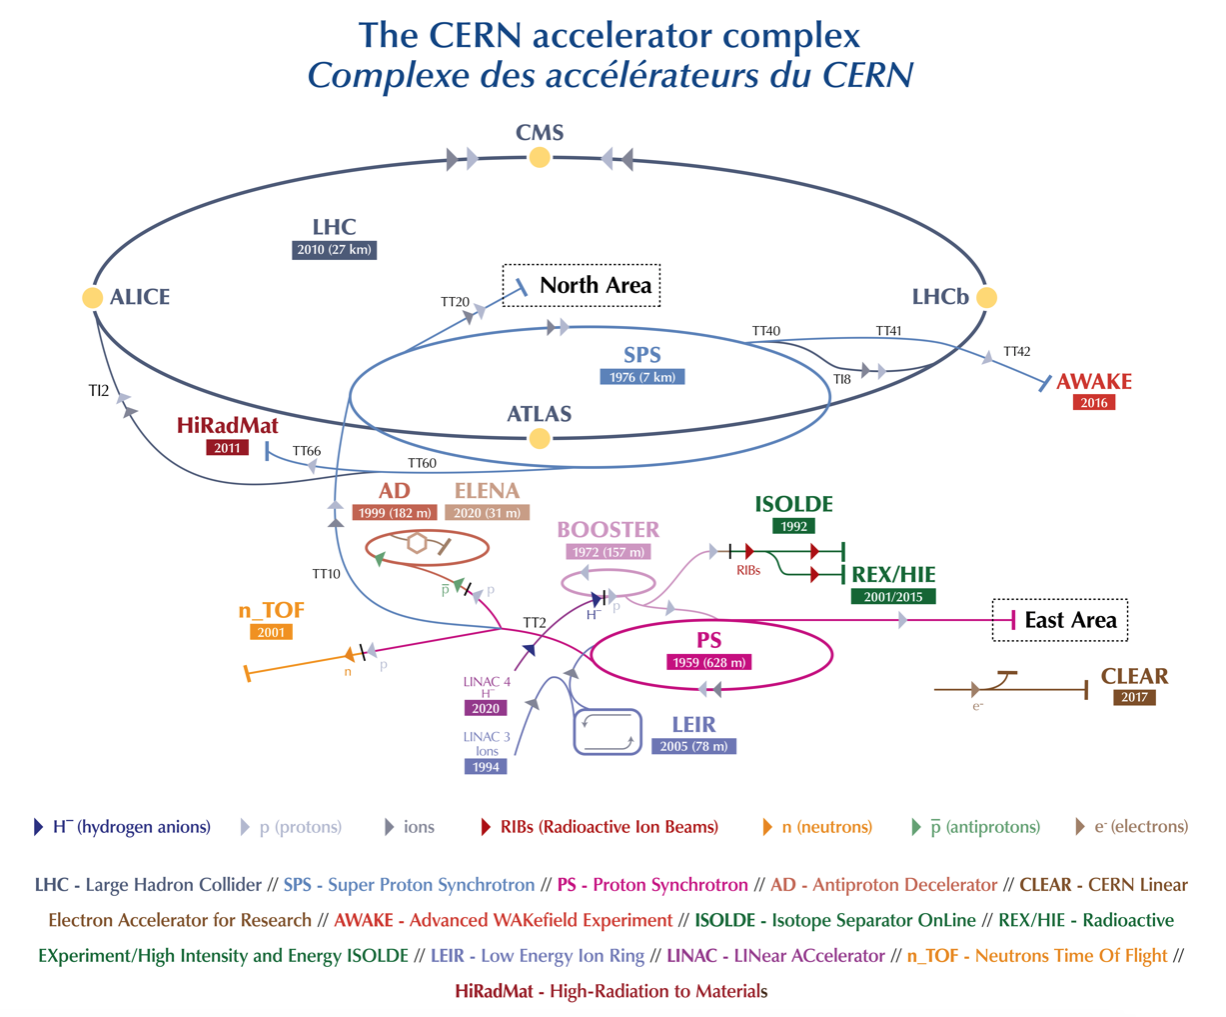
\includegraphics[width=1.05\textwidth]{Images/ATLAS/cernAcc}}
  \caption{The complete accelerator complex of CERN for Run 3 \cite{CERNAcc}.}
  \label{fig-CernAccSys}
\end{figure}

The operation of the \gls{lhc} is split into dedicated \textit{runs} of data taking separated by \textit{shutdowns} to maintain or upgrade the infrastructure. Key metrics about these runs from the point of view of the ATLAS experiment are displayed in Table~\ref{tbl:LHCATLASperf}. Run 2 operated at a larger centre-of-mass energy ($\sqrt{s}$) and higher average instantaneous luminosity $\mathcal{L}$ than Run 1, with the ongoing Run 3 yet again pushing up the limit.\\

{
\vspace{-1cm}
\begin{table}[!htbp]
  \begin{center}
      \renewcommand{\arraystretch}{1.2}
    %\resizebox{0.99\textwidth}{!}{
      \begin{tabular}{cc|cccc} \hline \hline 
        & Year & $\sqrt{s}$ [TeV] & $\langle \mu \rangle$ &  Luminosity $\mathcal{L}$ [cm$^{-2}$s$^{-1}$] & $\int\mathcal{L}$ [fb$^{-1}$] \\ \hline
        Run 1 & 2010 - 2012 & 7-8    & 18 & 0.8 $\times$ $10^{34}$    & $26.4$ \\
        Run 2 & 2015 - 2018 & 13     & 34 & 1-2 $\times$ $10^{34}$  & $140.1$ \\
        Run 3 & 2022 - 2025 & 13.6     & 50 & 2 $\times$ $10^{33}$    & $65$ \\

        \hline\hline
      \end{tabular}
    %}
    \caption{Metrics on the accelerator performance of the LHC in the different runs of data taking. The reported values correspond to those recorded by the ATLAS experiment \cite{ATLAS:run1Lumi, ATLAS:2022hro, ATL-DAPR-PUB-2023-001}. Numbers for the ongoing Run 3 are preliminary, with the integrated luminosity listed considering events recorded until July 2023. The number of interactions per bunch crossing averaged over each run is displayed as $\langle \mu \rangle$.}
    \label{tbl:LHCATLASperf}
  \end{center}
\end{table}
}

The average instantaneous luminosity $\mathcal{L}$ measures the quantity of data collected from the relation
\begin{equation}
  \frac{dN}{dt} = \mathcal{L} \times \sigma
\end{equation}
relating the event rate of a particular process to its cross-section $\sigma$. The instantaneous luminosity is a machine parameter: it depends on the design and the operation of the accelerator. It is calculated from
\begin{equation}
  \mathcal{L} = \frac{N_1N_2N_bf}{4\pi\sigma_x\sigma_y}
\end{equation}
where $N_1$ and $N_2$ are the number of protons in each bunch, $N_b$ the number of bunches, $f$ is the collider revolution frequency, and $\sigma_x$ and $\sigma_y$ are the geometrical extensions of the beam density distribution in the $x$- and $y$-direction. The integrated luminosity $\int \mathcal{L}\, dt$ measures the number of events collected over a certain period, often expressed in units of inverse \textit{barn} b$^{-1}$, where 1 b $= 10^{-28}$ m$^{2}$. For Run 2, the total luminosity recorded by ATLAS corresponds to 140.1 $\pm$ 1.2 fb$^{-1}$, with a small uncertainty of 0.83 \% \cite{ATLAS:2022hro} thanks to a complex measurement involving luminosity-dedicated detectors such as LUCID-2 \cite{Avoni_2018}. Figure \ref{fig-atlasLumiPileup} shows the cumulative distribution of the integrated luminosity during Run 2, jointly with another important machine parameter: the average number of interactions per bunch crossing $\langle \mu\rangle$.

\begin{figure}[!h]
  \centering
  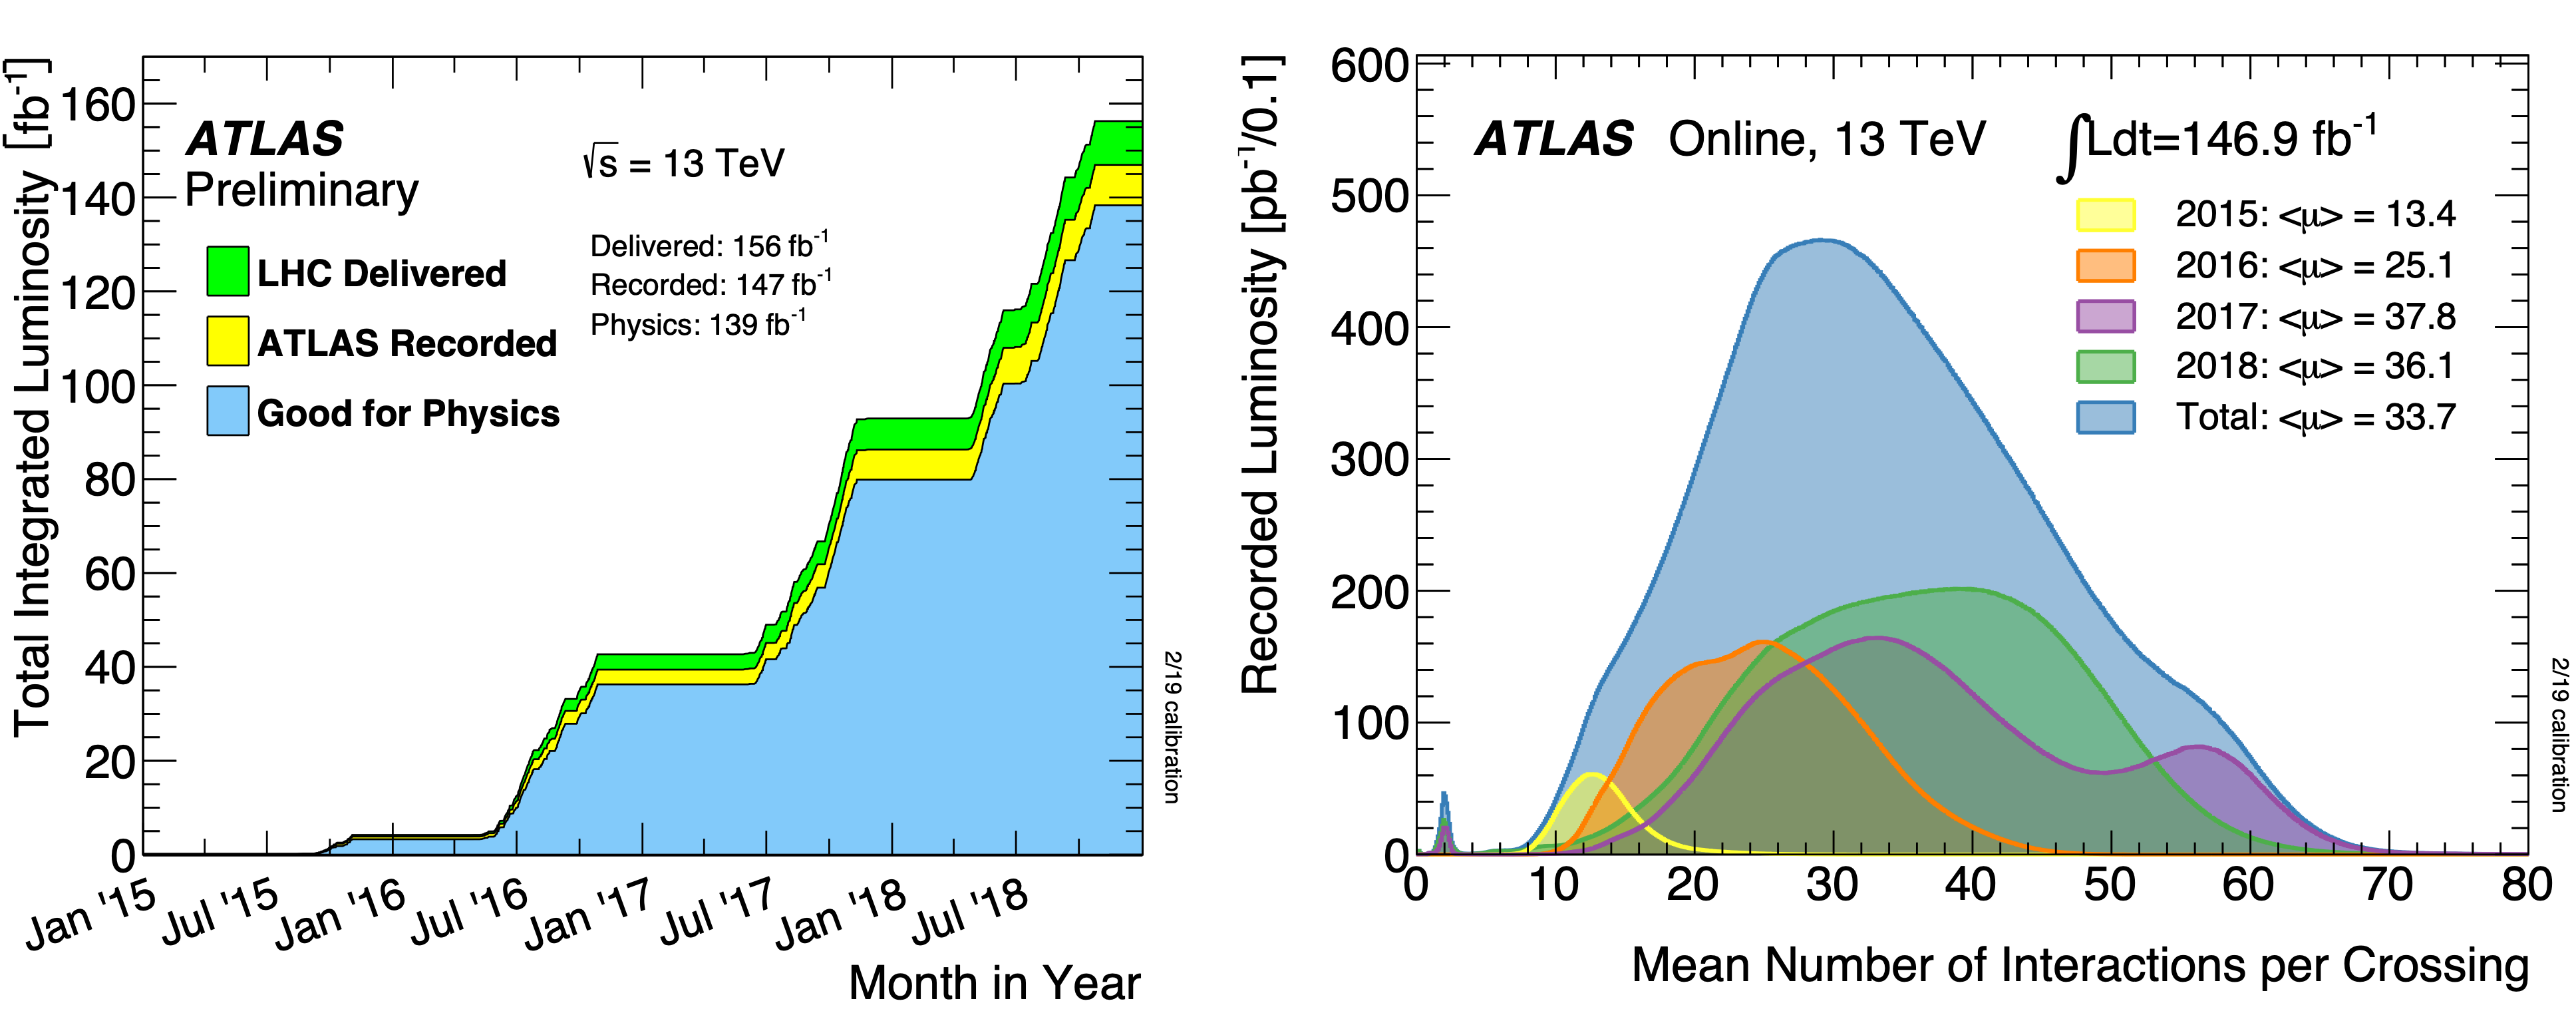
\includegraphics[width=\textwidth]{Images/ATLAS/recoATLAS.png}
  \caption{The ATLAS cumulative integrated luminosity delivered, recorded, and useful for physics (left) and the average luminosity-weighted pile-up distribution (right) during Run 2  \cite{PubAtlasLumi}. The luminosities listed correspond to an early calculation that was corrected in Ref. \cite{ATLAS:2022hro}.}
  \label{fig-atlasLumiPileup}
\end{figure}

\paragraph{}The main event during the collisions of the proton bunches is the inelastic hard scattering where most of the energy transfer occurs. Other protons in the bunches can have softer interactions leading to background activity referred to as \textit{\gls{pu}}. Two types of pile-up are distinguished: \textit{in-time \gls{pu}} when the soft interaction is from protons in the same bunch as those involved in the hard scattering, and \textit{out-of-time \gls{pu}} if the protons are from bunch-crossings just before or after the collision of interest. The \gls{lhc} separates bunches by a 25 ns delay, corresponding to a machine frequency of 40 MHz. To control the luminosity, the angle of attack of the beams are tweaked so that their geometrical overlap measured by $\sigma_x$ and $\sigma_y$ at the point of impact is tunable. Having more head-on collisions leads to a larger overlap and a higher luminosity at the price of more \gls{pu}. 

\section{The ATLAS Detector}\label{sec-ATLASDet}
The ATLAS Collaboration maintains and operates the eponymous cylindrically shaped multi-layered detector, lying 100 m underground with a length of 45 m and a 26 m diameter \cite{TheATLASCollaboration_2008}, as presented in Figure~\ref{fig-AtlasDec}. The experiment is designed to probe a broad range of physical phenomena. Aiming to be as hermetic as possible, the detector wraps around the interaction point, with the barrel forming the central part of the cylinder and the endcaps closing the geometry at its extremities. Essential requirements in the technical design had to be met to manage the extreme event rate by requiring a fast response from radiation-hard sensors with state-of-the-art readout electronics in combination with good spatial and temporal resolution to disentangle the effect of pile-up. 

\begin{figure}[!h]
\centering
\hspace{-1.25cm}
\makebox[\textwidth][c]{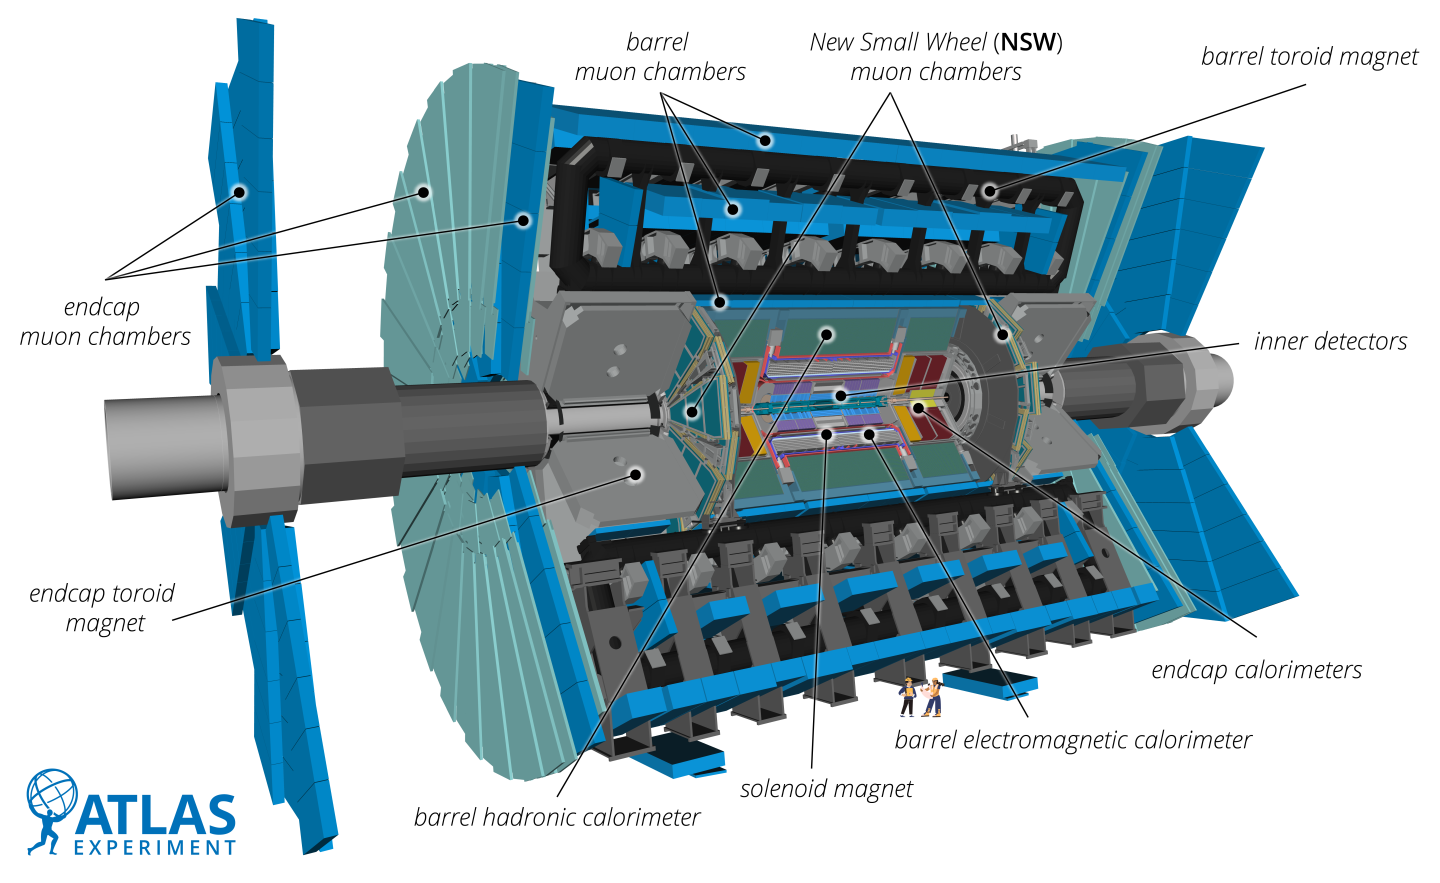
\includegraphics[width=1.08\textwidth]{Images/ATLAS/atlasDet.png}}
\caption{Cut-away view of the ATLAS detector \cite{ATLASschematics}.}
\label{fig-AtlasDec}
\end{figure}

The coordinate system adopted in ATLAS is described in Figure \ref{fig-AtlasCoord}: the $x$-axis points to the centre of the \gls{lhc} ring, the $y$-axis points upwards, and the $z$-axis is in the longitudinal direction along the beamline, anti-clockwise when viewed from atop. The azimuthal angle $\phi$ is defined in the transverse plane $x-y$, and the polar angle $\theta$ is measured upwards from the beam-axis. The transverse momentum \pt\ of a particle is obtained from its momentum vector $\boldsymbol{p} = (p_x, p_y, p_z)$ of magnitude $p$ as \pt\ $=p \sin\theta = \sqrt{p_x^2 + p_y^2}$. This projection plays a crucial role as the momentum's longitudinal component $p_z$ is not fully resolvable due to the openings for the beamline and the interacting partons carrying only a fraction of the original proton momenta. Only the transverse momentum can therefore be reliably measured. Since the partons are mostly longitudinally boosted, the transverse momenta in an event are approximately balanced. The rapidity $y$ of a particle is expressed as 
\begin{equation}
  y = \frac{1}{2} \ln \left(\frac{E + p_z}{E - p_z}\right)
\end{equation}
with $E$ and $p_z$ the energy and longitudinal momentum of the particle. In the ultrarelativistic limit, when $p >> m$, the rest mass is negligible and $E \approx p$. In this case, the rapidity $y$ is well approximated by the experimentally reconstructable pseudo-rapidity $\eta$:
\begin{equation}
  \eta = -\ln \left(\tan \frac{\theta}{2}\right).
\end{equation}
At high energies, $\Delta \eta$ becomes approximately invariant under Lorentz boosts along the $z$-axis. The pseudo-rapidity is often combined with the azimuthal angular aperture $\Delta \phi$ to define the angular separation $\Delta R$ between two objects as 
\begin{equation}\label{eq-def-deltaR}
  \Delta R = \sqrt{\Delta \phi^2 + \Delta \eta^2} =  \sqrt{\Delta (\phi_2 - \phi_1)^2 + \Delta (\eta_2 - \eta_1)^2}.
\end{equation}

\begin{figure}[!h]
  \centering
  %\hspace{+0.5cm}
  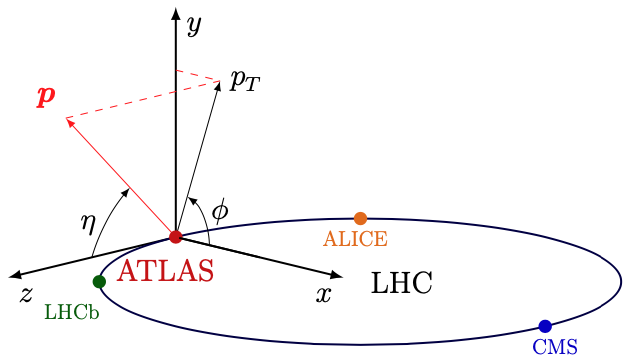
\includegraphics[width=0.6\textwidth]{Images/ATLAS/atlasCoor.png}
  \caption{The ATLAS coordinate system \cite{Strong:2020mge}.}
  \label{fig-AtlasCoord}
\end{figure}

As depicted in Figure~\ref{fig-AtlasDec}, ATLAS is composed of many subdetectors measuring information in the range $|\eta|<  2.5$, with some specialised subdetectors such as the calorimeters extending further. An essential feature of the detector is its magnetic field. In ATLAS, this is provided by four superconducting magnets: a Central Solenoid generates a 2 T axial magnetic field used by the central trackers, and a tangential magnetic field of about 1 T at the muon detectors is achieved by the Barrel Toroid and the two Endcap Toroids. A $q$-charged particle of momentum $p$ is deflected by a magnetic field $B$ due to the Lorentz force, leading to a relation between the radius of curvature $R$ of the trajectory and the momentum $p$ such that 
\begin{equation}
  p_{\perp} = 0.3 \, qBR \, [\text{GeV}/c],
\end{equation}
where $p_{\perp}$ is the magnitude of the momentum perpendicular to the magnetic field $\boldsymbol{B}$, and $q$ is expressed in the unit of proton charge. Therefore, by measuring the curvature, the component of the momentum transversal to the magnitude $B$ can be inferred. Higher magnetic fields induce larger curvature simplifying the measurement of $R$ and improving the resolution of $p_{\perp}$. \\ 

The rest of this chapter reviews the different subdetectors of ATLAS and introduces some common reconstruction methods that are relevant to the work presented in this thesis. 

\subsection{The Inner Detector Tracker}
The detector placed closest to the beam crossing point is the \gls{id} \cite{CERN-LHCC-97-016}. This tracker covering the range $|\eta| < 2.5$ in a radius of 3 cm to 1 m is designed to record hits in silicon semiconductors or straw tubes from the passage of charged particles so that their trajectory or \textit{track} can be reconstructed from the combined signature. The powerful 2 T magnetic field of the Central Solenoid enables this detector to measure both the charge and the momentum of charged particles. The \gls{id} combines three subsystems, represented in Figure \ref{fig-AtlasDecID}. 

\begin{figure}[!h]
  \centering
  \hspace{-1.25cm}
  \makebox[\textwidth][c]{\includegraphics[width=1.1\textwidth]{Images/ATLAS/ATLASinDecComb.png}}
  \caption{The Inner Detector of ATLAS \cite{ATLASschematics}.}
  \label{fig-AtlasDecID}
\end{figure}

First, the high-granularity \textit{Pixel Detector} covers the innermost region with three barrel and three endcap layers, for a total of 80 million sensitive semiconductor pixels \cite{CERN-LHCC-97-016, Potamianos:2015lar}. During Run 2, an additional \textit{\gls{ibl}} with 12 million pixels was added at a radius of 33 mm \cite{Capeans:1291633}. This detector gives robust and precise tracking performance and plays a major role in flavour tagging, as described in Chapter~\ref{chap-ftag}. The pixel dimensions range from 50 $\times$ 400 $\mu$m$^2$ in the Pixel Detector to 50 $\times$ 250 $\mu$m$^2$ in the \gls{ibl}, where the smaller dimension is used for the $R\phi$ measurement. The geometrical position resolution delivered is of 10 $\mu$m (67 $\mu$m) in the transverse $R\phi$ plane ($z$-direction) \cite{Pernegger_2015, ATL-INDET-PUB-2016-001}. \\

The \textit{\gls{sct}} is the next detector, constructed by arranging pairs of silicon microstrips layers into modules assembled into 4 concentric barrel layers and 9 disks in each endcap \cite{AHMAD200798, CERN-LHCC-2017-005}. The resolution is typically of 17 $\mu$m in $R\phi$ and 580 $\mu$m in $z$ \cite{ATLASSCT}. \\

The final system is the \textit{\gls{trt}}, a gas-based straw-tube tracker aiding track reconstruction by delivering numerous hits \cite{TheATLASTRTcollaboration_2008}. Approximately 300,000 drift tubes of a 4 mm diameter filled with a mixture of argon and xenon are arranged along the beamline in the barrel and radially in the endcaps. Each tube is fitted with a conducting wire at its centre and the surface is electrically charged, so that the passage of a charged particle ionises the gas leading to a measurable signal. Polyethylene is placed between the tubes to encourage the emission of transition radiations from relativistic particles proportionally to their Lorentz boost $\gamma \sim E / m$. The \gls{trt} is used for both tracking and electron and pion identification, by reconstructing the mass of the charged particles from the amount of $\gamma$-radiation. For tracking, the position resolution provided is 130 $\mu$m in the $R\phi$ plane for the barrel and the $z-\phi$ plane in the endcaps \cite{Vogel:1537991}. \\

Altogether, the track inverse transverse momentum resolution of the ATLAS \gls{id} is
\begin{equation}
  \sigma(1 / p_T) = 0.36 \oplus \frac{13}{p_T \sin\theta} \text{TeV}^{-1}
\end{equation}
where $\oplus$ denotes a sum in quadrature \cite{TheATLASCollaboration_2008}. This corresponds to a relative error of about 0.01\% for a track with \pt\ $\sim$ 500 MeV, and 4\% at a \pt\ $\sim$ 100 GeV.

\subsection{Electronic and Hadronic Calorimeters}
Covering the $|\eta| < 4.9$ region, calorimeters collect the energy of all interacting particles, neutral and charged. The system is composed of an \gls{ecal} and a \gls{hcal} both covering the $|\eta| < 3.2$ region and a forward calorimeter for the $3.2 < |\eta| < 4.9$ region \cite{TheATLASCollaboration_2008}, as displayed in Figure~\ref{fig-AtlasDecCalo}.\\

The \gls{ecal} is designed to collect the energy of electrons and photons and contributes to the measurement of the energy of jets. The active material is LAr, with absorbing plates of lead used as passive material to encourage \textit{bremsstrahlung} $e \rightarrow e\gamma$ and pair production from photons $\gamma \rightarrow e^+e^-$. The \gls{ecal} has a depth of at least 22 $X_0$, where the unit of \textit{radiation length} $X_0$ tracks the distance for an electron to retain only 1/$e$ of its original energy. The energy resolution is parametrised into three terms representing the sampling term, the electric noise, and a constant contribution for miscalibrations, summed in quadrature as \cite{Cavallari_2011}
\begin{equation}
  \frac{\sigma_E^{\text{ECAL}}(E)}{E} = \frac{10\%}{\sqrt{E}} \oplus \frac{0.17 [\text{GeV}]}{E} \oplus 0.7\%,
\end{equation}
giving an energy resolution between $\sim$0.5\% for 10 GeV electrons, and $\sim$ 0.6\% for 60 GeV photons.\\

\begin{figure}[!h]
  \centering
  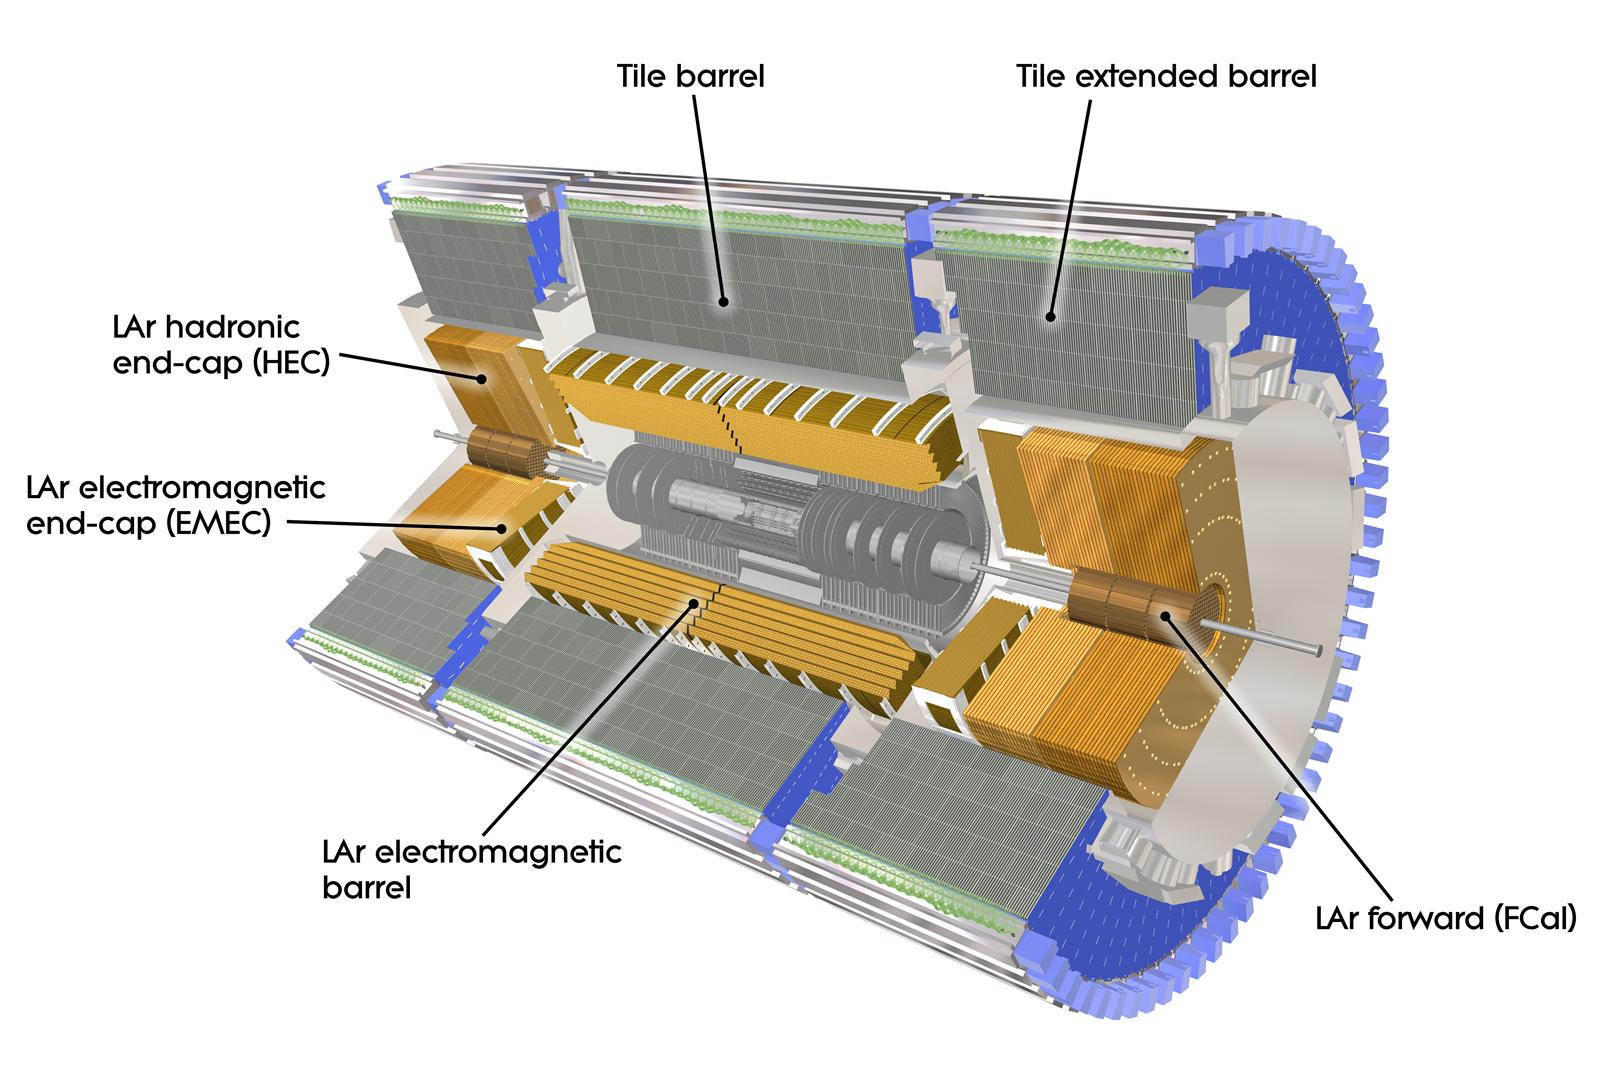
\includegraphics[width=\textwidth]{Images/ATLAS/ATLASCalo.jpg}
  \caption{The calorimeter systems of ATLAS \cite{ATLASschematics}.}
  \label{fig-AtlasDecCalo}
\end{figure}

The \gls{hcal} is designed to capture the energy of hadronic showers, with LAr as active material for the endcap and forward calorimeters and scintillating plastic tiles for the barrel. As passive material, the endcaps use copper plates, the forward calorimeters use copper and tungsten, and the tile calorimeter in the barrel uses steel. The depth of the hadronic calorimeter is approximately $10 \lambda$, where $\lambda$ is the nuclear interaction length tracking the average distance before a hadron interacts with a nucleus. The calorimeters collect the majority of the energy of hadrons, with an \gls{hcal} resolution expressed as \cite{Cavallari_2011}
\begin{equation}
  \frac{\sigma_E^{\text{HCAL}}(E)}{E} = \frac{52.9\%}{\sqrt{E}} \oplus 5.7\%.
\end{equation}
This translates into a resolution of $\sim$17\% ($\sim$6\%) at energies of $\sim$10 GeV ($\sim$100 GeV).

\subsection{Muon Detection Systems}
\begin{figure}[!h]
  \centering
  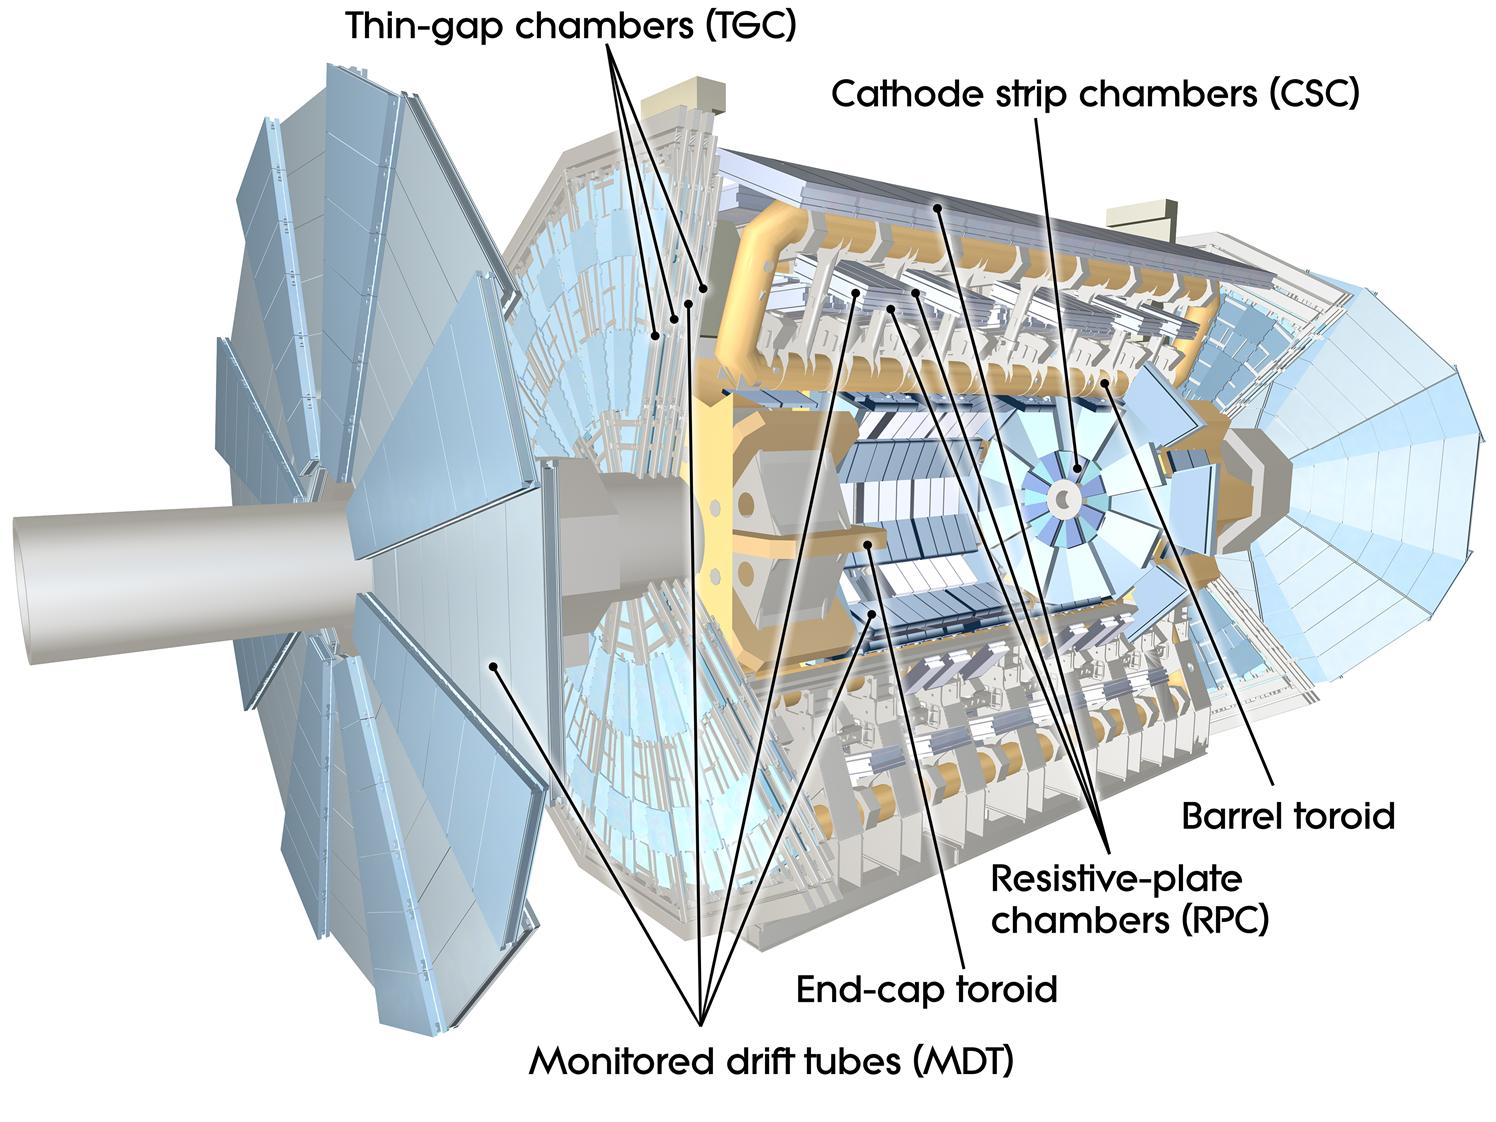
\includegraphics[width=0.9\textwidth]{Images/ATLAS/ATLASMuon.jpg}
  \caption{The muon detectors of ATLAS \cite{ATLASschematics}.}
  \label{fig-AtlasDecMuon}
\end{figure}
Muons require dedicated detection systems to be efficiently and precisely reconstructed. While they leave good tracks in the \gls{id}, muons do not leave much energy in the calorimeters due to their high mass suppressing bremsstrahlung radiations. For this reason, the outmost subdetectors of ATLAS are specially designed to be sensitive to muons. The \gls{ms}, shown in Figure~\ref{fig-AtlasDecMuon}, is a dedicated muon tracking system that also provides an effective triggering hardware, as described later in this chapter. The muon tracker is composed of drift tubes split between the barrel region for $|\eta| < 1.2$ and the endcaps $1.2 < |\eta| < 2.7$, with cathode strip chambers in the inner layers of the endcaps. The trigger system relies on resistive-plate chambers in the barrel and thin-gap chambers in the endcaps. To improve momentum and charge measurements from the reconstructed tracks, powerful superconducting toroidal magnets are used to deflect muons in the \gls{ms}. The resolution on \pt\ is measured to be of $\sim 2.3$\% (2.9\%) for muons from $Z$ decays in the central (forward) region \cite{atlasMuonPTReco}.

\section{Operation and Reconstruction with the ATLAS Detector}\label{chap-atlas-reco}
For physics-quality data taking, the different subdetectors of ATLAS must be performing according to specifications. In operation, the event rate produced by the \gls{lhc} in the heart of the ATLAS detector is 40 MHz, due to the 25 ns bunch-crossing. This unfortunately leads to a data generation rate that is too high for the computing resources available, requiring the Collaboration to design specific approaches to reduce the rate to a manageable level \cite{Nedden_2017}. This is the task of the trigger system, which is described in this section. Events that pass the trigger thresholds are stored and must be further analysed to reconstruct the physics processes from the low-level measurements performed by the different subdetectors: this is the task of reconstruction, the last subject described in this chapter for object types relevant to the presented work. This latter step is performed thanks to the extensive ATLAS software \cite{ATL-SOFT-PUB-2021-001, ATL-SOFT-PUB-2020-001}, exploiting the specific signatures of the different detected particles as schematised in Figure~\ref{fig-ATLASdetect}.

\begin{figure}[!h]
  \centering
  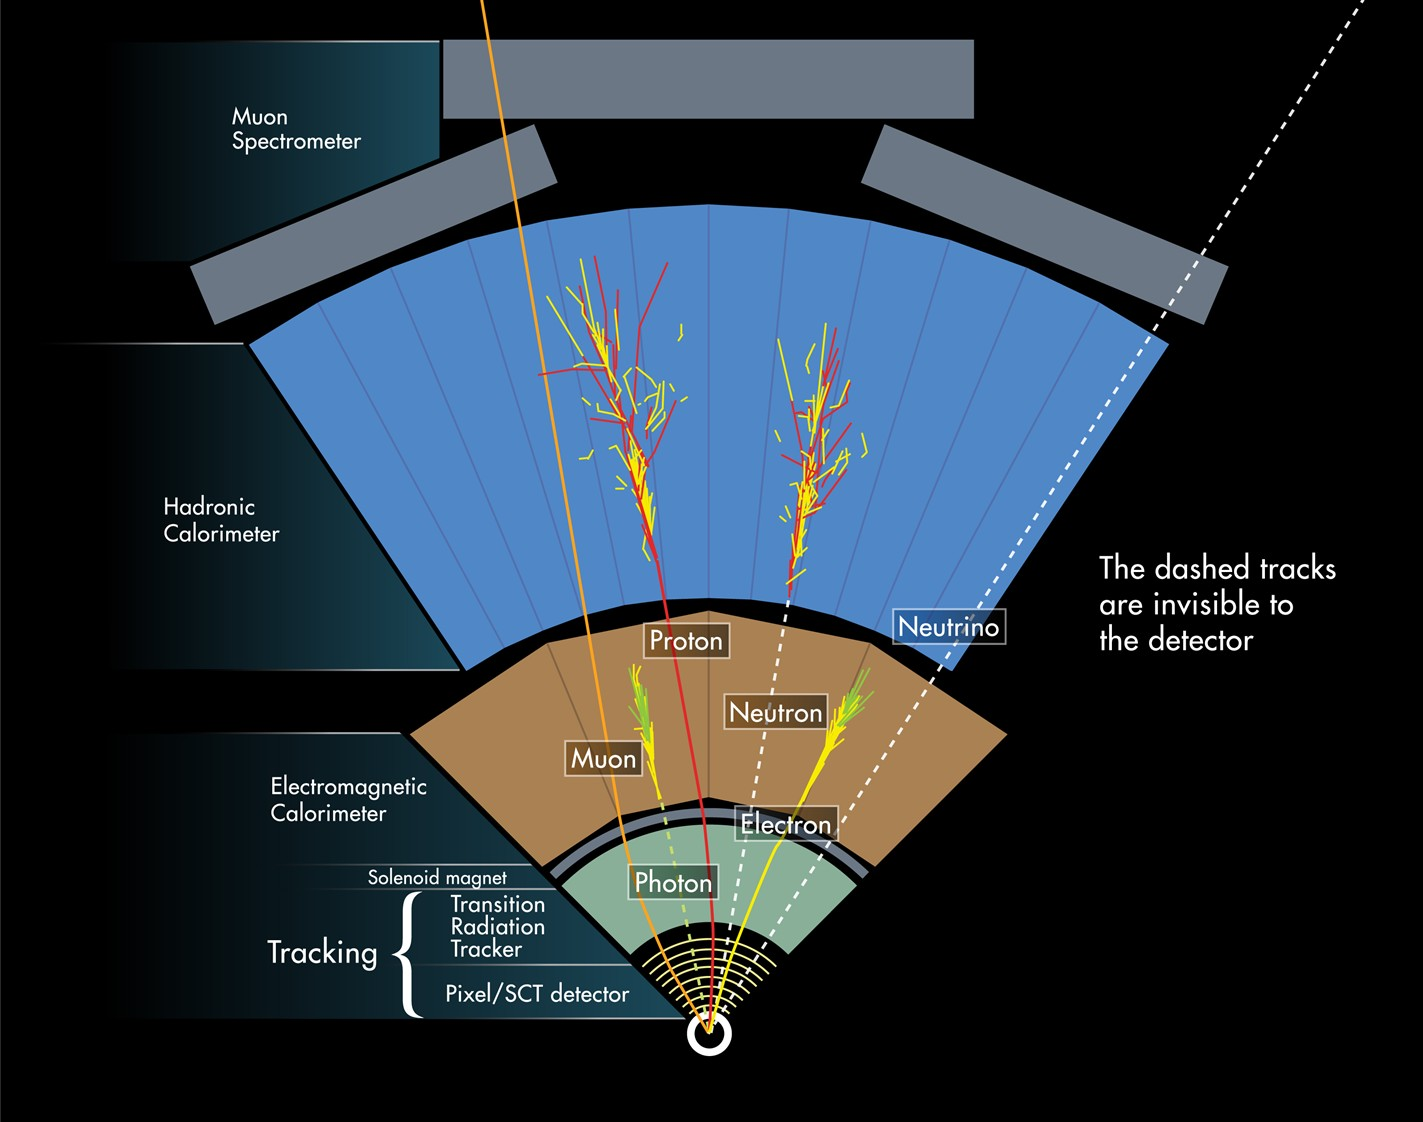
\includegraphics[width=0.8\textwidth]{Images/ATLAS/ATLASdetection.jpg}
  \caption{Schematics of different particles signatures in the ATLAS detector \cite{Pequenao:1505342}.}
  \label{fig-ATLASdetect}
\end{figure}

\subsection{Trigger System}\label{sub-sec-trigger}
The ATLAS trigger system relies on a hierarchical approach to progressively reduce the data rate and select events deemed interesting for physics. Firstly, the Level-1 (L1) trigger is built on fast electronic hardware accessing coarse information to reduce the rate to 100 kHz in $\sim$ 2.5 $\mu$s. This is followed by the High-Level Trigger (HLT) that runs on a farm of 40,000 \glspl{cpu} to implement a finer software-based selection, bringing the rate down to a 1.2 kHz or 1.2 GB/s suitable for data storage \cite{TriggerATLAScollaboration_2020}. In this process, gradually more complex information is accessed by dedicated readout and measurement systems. Some commonly used triggers are based on signatures of electrons, muons, missing transverse energy, and $b$-jets. Different trigger menus are designed by the Collaboration, with dedicated data-taking periods for each setup. Analyses can then select data collected with the most optimal trigger stream for the specific signatures sought. 

\subsection{Low-Level Signatures: Tracks, Vertices, and Clusters}\label{sec-atlas-lw}
Low-level signatures are used in higher-level reconstruction processes to identify physics objects, such as electrons and jets. Three types are described here: the trajectory of charged particles called \textit{tracks}, the construction of vertices, and the formation of calorimeter clusters. \\

Tracks are the reconstructed trajectory of charged particles through the detector from the collected localised energy deposits called \textit{hits}. With denser pile-up activity, the number of hits in a single event becomes significant, making track reconstruction a challenging computational problem \cite{ATL-PHYS-PUB-2015-006, ATLAS-tracks-algo,}. The trajectories are curved thanks to the previously described superconducting magnets. From a set of hits, tracks are fitted inside-out \cite{ATLAS-tracks-algo}: clusters of three hits in the Pixel or \gls{sct} detectors are first identified as \textit{seeds}, with additional hits associated by a combinatorial Kalman Filter \cite{10.1115/1.3662552} based on compatibility criteria with the initial track. Hits can initially be shared by several tracks, with the ambiguity resolved later when the reconstructed tracks are ranked by quality and $\chi^2$-fits are performed to quantify the best possible association while favouring high \pt\ tracks. The process is then extended to the \gls{trt} from the outside-in, and followed by additional quality criteria such as requiring tracks to have a \pt\ > 500 MeV in $|\eta| < 2.5$, a minimum of 7 hits in the Pixel and \gls{sct}, at most one missing hit (hole), and at most two shared hits. Tracks are parametrised by the longitudinal (along $z$) and transversal (in the $x-y$ plane) \glspl{ip}, respectively $z_0$ and $d_0$, measuring the distance from the \gls{pv} to the point of closest approach of the track (the perigee). \\

If a reconstructed charged particle is produced in the hard scattering event, its trajectory leads back to a location called the \textit{\glsfirst{pv}} \cite{ATLAS:2016nnj} where the $pp$ interaction occurs. If the particle is produced in a subsequent decay, the point of emanation can sometimes be distinguished and is labelled \textit{\gls{sv}} \cite{Kostyukhin:685551}. Reconstructing the vertices is crucial for the physics programme of the Collaboration. The primary vertex is identified from a seed vertex first on the set of all well-reconstructed tracks \cite{ATL-PHYS-PUB-2015-026}. The vertex position is then iteratively refined by removing tracks incompatible with the reconstructed vertex and refitting, until quality criteria are met. Discarded tracks are then used to identify secondary and tertiary vertices. The primary vertex is the one with the highest sum of squares of contributing track transverse momenta \pt. \\

In the ATLAS calorimeters, \textit{clusters} are identified by grouping cells with energy deposits matching specific criteria, either from the \textit{sliding window} or \textit{topocluster} algorithms \cite{Lampl:1099735}. The former generates fixed-size rectangular clusters by translating a window to maximise the transverse energy $E_T$ measured. The latter clusters neighbouring cells based on a signal-to-noise criterion. As the sliding window method is easier to calibrate, it is used in electron, photon, and hadronic-$\tau$ reconstruction. Topoclusters are robust against noise and therefore used for jet and missing transverse energy reconstruction.

\subsection{Electrons}\label{sec-atlas-el}
Electrons leave signatures in the \gls{id} and \gls{ecal}. In the central region $|\eta| < 2.5$, electrons are identified and reconstructed with both subdetectors. The forward region $2.5 < |\eta| < 4.9$ is only covered by the calorimeters, and the shape of the shower is used to identify electrons. Here, only centrally produced \textit{prompt} electron reconstruction is described, where \textit{non-prompt} electrons are not produced from the main physics process but through later decays or interactions with the detector itself. Since photons, pions, and jets can be mistaken as electrons, identification and isolation criteria must be implemented to provide high-purity electron candidates for analyses. The reconstruction relies on calorimeter clusters and track information. Tracks are matched to clusters with the expected energy loss taken into consideration. The track is extrapolated to ensure compatibility with the cluster barycentre, and the process is run again with more stringent conditions after refitting the matched tracks. A prompt electron is required to have a track matched to the \gls{pv}. The absence of precision hits or a matched track leads to considering the calorimeter clusters as a photon deposit. Converted photons are allowed hits in the outer layers of the \gls{id}. Photons can however be mistaken as electrons due to the photon-conversion process, where $\gamma \rightarrow e^+e^-$. \\

To further distinguish prompt electrons from non-prompt electrons and photons, a likelihood-based identification algorithm built on a \glsfirst{mva} discriminant is deployed \cite{Aaboud:2657964}. Features exploited include the number of hits in each tracker layer, the track \glspl{ip}, and some calorimeter cluster parameters. Several operating points that are progressively more selective are defined on the \gls{mva} discriminant, from \textit{Very Loose}, \textit{Loose}, \textit{Medium}, to \textit{Tight}. Prompt electron candidates are required to be isolated from other tracks and energy deposits, with specific isolation criteria that are either \gls{id}- or calorimeter-based. In the former case, the sum of tracks \pt\ in a $\Delta R$ cone around the electron is used, while the latter analyses the sum of energy deposits in a calorimeter cone around the electron cluster. As further described in Chapter~\ref{sec-unc}, the efficiencies of the electron reconstruction, including identification and isolation, are estimated by comparing the measured and simulated measurements of the $Z\rightarrow e^+e^-$ and $J/\psi\rightarrow e^+e^-$. 

\subsection{Muons}\label{sec-atlas-mu}
The \gls{ms} is the main detector to identify muons, with other subdetectors such as the \gls{id} used to reconstruct the properties of these leptons. Muons indeed leave tracks in the \gls{id} and some energy deposits in the calorimeters. The signatures in the different subdetectors are combined to reconstruct muon candidates. In the \gls{ms}, tracks are constructed from a fit of the successive hits in the different chambers. \textit{Combined muons} are defined by matching a track in the \gls{ms} to a track in the \gls{id}, with additional information from the calorimeters. Prompt muons are rejected from background-produced muons (such as in the decay of a $b$-hadron) by specific criteria targeting discrepancies in the \pt\ between the \gls{ms} and \gls{id}. Increasingly selective operating points are defined to identify muons as \textit{Loose}, \textit{Medium}, \textit{Tight}, and \textit{High-\pt}. Isolation requirements are applied similarly to the electron case, either track- or calorimeter-based in a $\Delta R$ cone around the candidate muons. The calibration of muons is performed similarly to the electrons, on $Z\rightarrow \mu^+\mu^-$ and $J/\psi\rightarrow \mu^+\mu^-$ samples.

\subsection{Jets}\label{sec-atlas-jets}
Quarks and gluons are the most commonly produced particles in a hadron collider. As described in Chapter~\ref{chap-theory}, these particles carry colour charges and therefore undergo hadronisation when produced to neutralise their free colour. This complex phenomenological process leaves a unique signature in the detector: a spray of particles emitted within the original parton direction called a \textit{jet}. Electrically charged and neutral particles are contained within jets, with most of the energy deposited in the hadron calorimeters. These aggregated objects are constructed by applying a clustering algorithm on tracks and/or calorimeter clusters, depending on the jet definition. \\ 

The most notorious clustering method is the anti-$k_T$ algorithm, thanks to the robustness of the defined jets to collinear splitting and additional soft emissions \cite{Cacciari:2008gp}. The algorithm starts by considering high-momentum objects, after which softer objects are considered and potentially added to grow the jets or start a new jet. Two objects are considered at a specific step of the algorithm: the seed object $i$, either the highest momentum object or the jet in construction, and the currently unassigned highest transverse momentum object $j$. Two distances are evaluated when considering whether to cluster these objects
\begin{equation}
  d_{ij} = \min\left(\frac{1}{k_{Ti}^2}, \frac{1}{k_{Tj}^2} \right) \frac{\Delta R_{ij}^2}{R^2} \quad \text{and} \quad d_{iB} = \frac{1}{k_{Ti}^2}.
\end{equation}
The first distance, $d_{ij}$, combines the angular apperture $\Delta R_{ij} = \sqrt{(\eta_i - \eta_j)^2 + (\phi_i - \phi_j)^2}$ between $i$ and $j$ with the transverse momentum $k_T$ of the two objects and a fixed \textit{radius} parameter $R$. This distance defines a radius limiting the size of the jet cone. It is compared to the second distance, $d_{iB}$, assessing the size of the already formed jet $i$. If $d_{ij} < d_{iB}$, $j$ is clustered with $i$ into a larger jet $i$, otherwise $i$ is identified as a jet and removed from consideration. The algorithm proceeds after updating the distances until all constituents are assigned. Typical radii for ATLAS are $R = 0.4$ and $R=1.0$, defining respectively small-$R$ and large-$R$ jets. The former is commonly used for quark and gluon jets, while the latter is employed to identify heavy object decay, such as $W$ or Higgs bosons. \\

Jets can be constructed from tracks, calorimeter clusters, or both. In ATLAS, several types of jets are deployed. The following types are all reconstructed with the anti-$k_T$ algorithm but clustering different objects:
\begin{itemize}[leftmargin=*]
\item PFlow jets combine particle-flow objects \cite{atlasPFLOWjet} with a radius $R$ = 0.4. These objects combine tracking information from the \gls{id} with the calorimeter clusters, leading to a better energy resolution at low \pt\ and lower pile-up contamination after calibration \cite{PhysRevD.96.072002}.
\item EMTopo jets are constructed from denoised topological calorimeter clusters called \textit{topoclusters}, based on the per cell energy significance $S_{\text{cell}} = E_{\text{cell}} / \sigma_{\text{cell}}$, where $E_{\text{cell}}$ is the energy and $\sigma_{\text{cell}}$ the expected noise level in the cell \cite{atlasEMTOpo}. The topoclusters are then used with the anti-$k_T$ method with a small (0.4) or large (1.0) radius.
\item Large-$R$ jets are built from topological calorimeter clusters with a radius $R = 1.0$. These jets are trimmed to remove the contributions from soft contamination, which is mainly due to \gls{pu} and \gls{ue} activity, leading to an improved mass resolution \cite{ATLAS:largeRjet}.
\item Track-jets are constructed with a \gls{vr} depending on the jet \pt, such that the wide cone used at low \pt\ ($R \sim 0.4$) becomes narrower at high \pt\ ($R \sim 0.02$). They are typically identified as sub-jets of a large-$R$ jet, to give access to the single-jet flavour tagging techniques described in Chapter~\ref{chap-ftag}.
\end{itemize}
PFlow and \gls{vr} jets are used to train the algorithms of Chapter~\ref{chap-ftag}, while EMTopo, large-$R$, and track-jets are used in the analysis of Chapter~\ref{chap-VH}. Jets are assigned a flavour based on the presence of an original parton within a $\Delta R = 0.3$ cone around the jet axis. Experimentally, the flavour is often determined based on the hadrons found within the jet, as described in detail in Chapter~\ref{chap-ftag}. \\

Jets benefit from an extensive calibration to correct their reconstructed properties such as the mass, the energy, and the jet axis. In particular, corrections to account for \gls{pu} activity and out-of-cone emissions and deposits are considered. Detector effects are also taken into account, such as differences between the electromagnetic and hadronic calorimeters and leakage out of the active regions. The \textit{\gls{jes}} calibration implements these corrections in successive steps \cite{ATLASjesjerMeas}: 
\begin{itemize}[leftmargin=*]
\item \textit{Origin}: the jet axis, initially constructed from the centre of ATLAS, is corrected to point from the \gls{pv}, and the reconstructed \pt\ is updated.
\item \textit{Pile-up}: both in-time and out-of-time pile-up leave additional energy deposits in the calorimeters. This is subtracted from the jet, first from an overall estimation based on the average \gls{pu} and then from the actual number of interactions and vertices in the event. 
\item \textit{Absolute}: absolute energy corrections dependent on the energy $E$ and $\eta$ are derived to match the data energy scale to the particle-level energy scale with dedicated simulation samples.
\item \textit{Eta inter-calibration}: the detector is not homogenous and the forward region measurements are typically less accurate. Corrections are applied to forward jets based on central jets ($|\eta|<1.4$).
\item \textit{Global sequential calibration}: energy leakage in the calorimeters is accounted for with a set of momentum corrections based on five different observables representing the jets shape and energy.  
\item \textit{In-situ calibration}: corrects any possible differences due to an incorrect description of the detector in the simulations by performing a fit to data in the dedicated measurement of a well-reconstructed object. Events from the following processes are used at increasing \pt\ scales: $Z+$jet events with the leptonic $Z$ decays, $\gamma$+jet, and \gls{qcd} multi-jet events.
\end{itemize}
The \gls{jes} is parametrised by \pt, and uncertainties are derived for analyses to include in their modelling. The \textit{Jet Energy Resolution (JER)} is then defined as $\sigma_{p_T}/p_T$, and also calibrated with uncertainties derived from a fit to di-jet events \cite{ATLASjesjerMeas}. Despite the \gls{jes} correction procedure, \gls{pu} jets can still be significant and a \gls{jvt} is used to reject this background \cite{ATLAS-CONF-2014-018}. This implements a 2D likelihood method built from track variables. From this discriminant, different selection criteria are derived as operating points with specific \gls{pu} jet rejections. 

\subsection{Taus}\label{sec-atlas-tau}
Taus are the heaviest generation of charged lepton, with a mass of 1.8 GeV slightly higher than that of $c$-quarks \cite{Tanabashi:2018oca}. Their lifetime is so short that they mostly decay within the beampipe. They leptonically decay 35\% of the time to neutrinos and an $e$ or a $\mu$, hence their hadronic decays are more frequent. The leptonic decays are hard to disentangle from prompt electrons and muons. Hadronic decays however leave a discernable signature reconstructed as a small-$R$ jet identified by a \glsfirst{rnn}, to disentangle them from \gls{pu} and \gls{qcd} jets \cite{ATL-PHYS-PUB-2019-033}. Different operating points are derived at specific efficiencies. 

\subsection{Missing Transverse Energy}\label{sec-atlas-met}
Some physics objects do not leave a signature in the detector, such as neutrinos. Their presence is not directly detectable but can be inferred thanks to the negligible initial \pt\ of the two interacting partons. Requiring the transverse energy \etm\ and momentum to be balanced, the missing transverse energy is calculated as the negative vectorial sum of the transverse momenta of objects, as
\begin{equation}
  \boldsymbol{E}_T^{\text{miss}} = - \sum_{\text{hard}} \boldsymbol{p}_T - \sum_{\text{soft}} \boldsymbol{p}_T,
\end{equation}
where the sum is decomposed into a \textit{hard} term englobing all high-level physics objects and a soft term including good-quality \gls{id} tracks associated with the primary vertex but not matched to a high-level physics object \cite{ATLASmetReco}. The performance of the reconstruction is measured by comparing simulations to data, with scale and resolution derived with uncertainties to be used by physics analyses. 